    % In Figure \ref{fig:case_1_c_2}, we observe blocks of $w'$ start inside blocks of $w$.

    \begin{figure}[ht!]  % 'htbp' suggests placement options
    \centering
    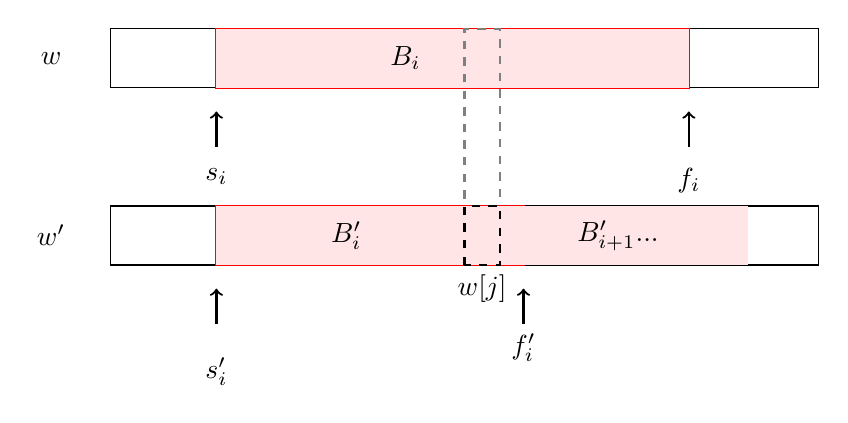
\begin{tikzpicture}[scale=1.5]
        % Main Rectangle w
        \draw (0,0) rectangle (6,0.5);
        \node at (-0.5, 0.25) {\(w\)};

        % Smaller Rectangle 1 - Border color red
        \draw[draw=red, thick] (0.9,0) rectangle (4.9,0.5);
        
        \draw[->, thick] (0.9,-0.5) -- (0.9,-0.2);
        \node[align=center, below] at (0.9,-0.6) {\(s_i\)};
        \draw[->, thick] (4.9,-0.5) -- (4.9,-0.2);
        \node[align=center, below] at (4.9,-0.6) {\(f_i\)};
        \fill[red!10] (0.9,0) rectangle (4.9,0.5);
        \node at (2.5,0.25) {$B_{i}$};


        % Dashed vertical line
        \draw[draw=gray, thick, dashed] (3.0,-1.5) rectangle (3.3,0.5);
        \node[align=center, below] at (3.15,-1.5) {\( w[j]\)};

        % Duplicate the structures for w' below
        % Offset for w' is -1.5 from w
        \begin{scope}[yshift=-1.5cm]
            \draw (0,0) rectangle (6,0.5);
            \node at (-0.5, 0.25) {\(w'\)};

            \draw[draw=red, thick] (0.9,0) rectangle (3.5,0.5);
            
            \draw[->, thick] (0.9,-0.5) -- (0.9,-0.2);
            \node[align=center, below] at (0.9,-0.7) {\(s'_i\)};
            \fill[red!10] (0.9,0) rectangle (3.5,0.5);
            \node at (2.0,0.25) {$B'_{i}$};
            
            \draw[->, thick] (3.5,-0.5) -- (3.5,-0.2);
            
            \node at (3.5,-0.7) {$f'_i$};

            % \draw[draw=red, thick] (3.5,0) rectangle (4.9,0.5);
            \fill[red!10] (3.5,0) rectangle (5.4,0.5);
            \node at (4.3,0.25) {$B'_{i+1}...$};
            
            \draw[draw=black, thick, dashed] (3.0,-0.0) rectangle (3.3,0.5);
        \end{scope}
    \end{tikzpicture}
    \caption{Compression for $w$ and $w'$ which $f'_{i+1}\geq j$.}
    \label{fig:case_1_c_2}
\end{figure}